\documentclass[12pt]{article}

\usepackage[margin=1in]{geometry}
\usepackage{amsmath,amsthm,amssymb}
\usepackage{nccmath}
\usepackage{mathtools}
\usepackage{mathrsfs}
\usepackage{enumitem}
\usepackage{physics}
\usepackage{slashed}
\usepackage{pdfpages}
\usepackage{float}

\usepackage{tikz}
\usetikzlibrary{calc,decorations.markings,patterns}

\graphicspath{ {./images/} }

\begin{document}

\title{Homework 3}
\author{Sean Ericson \\ Phys 663}
\maketitle

\section*{Problem 1}
\begin{enumerate}[label=(\alph*)]
    \item 
    \begin{figure}[h]
        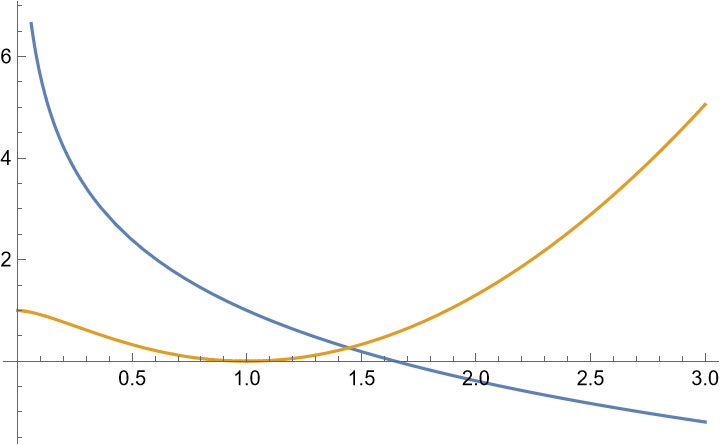
\includegraphics[scale=0.75]{S_T.PNG}
        \centering
        \caption{Example Plots of $S$ and $T$.}
        \label{fig1}
    \end{figure}
    Let $x = m_u / m_d$. Then,
    \begin{align*}
        S &= \frac{N_c}{6\pi}\left[1 - 2Y\ln x^2\right] \\
        T &= \frac{m_u^2N_c}{16\pi\sin^2\theta_W\cos^2\theta_Wm_Z^2}\left[1 + x^2 - \frac{2x}{x^2 - 1}\ln(x^2)\right]
    \end{align*}
    Now,
    \begin{align*}
        S = 0 \implies x = e^{Y/4} = x_0.
    \end{align*}
    $s$ is monotonically deceasing in $x$, so $S$ is positive when $x<x_0$ and negative when $x > x_0$. To show that $T$ is non-negative, it suffices to show that its minimum is $\ge 0$. The derivative of $T$ with respect to $x$ is (ignoring the constants out front)
    \[ \dv{T}{x} = 2x(3 - 4x^2 + x^4 + 4\ln(x))(x^2 - 1)^{-2}. \]
    Clearly the derivative has a zero at $x=0$. The value of the derivative at $x=1$ is undefined, but it's limit is 0 (see Mathematica printout). Any other zeros will be given by
    \begin{align*}
        \dv{T}{x} &= 0 \\
        \implies 2x(3 - 4x^2 + x^4 + 4\ln(x))(x^2 - 1)^{-2} &= 0 \\
        \implies 3 - 4x^2 + x^4 + 4\ln(x) &= 0
    \end{align*}
    For $x \ge\sqrt{2}$, the polynomial part is strictly increasing and the logarithm is positive, so there can be no other zeros. Hence, $x=1$ is the global minimum. The value of $T$ is undefined at $x=1$, but its limit is 0. Therefore, $T$ is always non-negative.
    
    \item Defining $m_u = m_d + \Delta$, we have that
    \begin{align*}
        S &= \frac{N_c}{6\pi} - \frac{2YN_c}{3\pi m_d}\Delta + O(\Delta^2) \\
        T &= \frac{N_c}{12\pi\sin^2\theta_W\cos^2\theta_Wm_Z^2}\Delta^2 + O(\Delta^3)
    \end{align*}
    (see Mathematica printout). Clearly, $T$ is suppressed in the $\Delta = 0$ limit.

    \item In the degenerate mass limit, $N_c = 6\pi S$. Then,
    \[ S_\text{new} = -0.01 \pm 0.07 \implies N_c = -0.2 \pm 1.3 \]
    I'm not really sure what the hint for this part of the problem is getting at. Given that this value of $S_\text{new}$ is 1 within uncertainty, it seems like this allows for a new extra heave generation of fermions with degenerate masses.
\end{enumerate}

\section{Problem 2}
\begin{enumerate}[label=(\alph*)]
    \item Using the given values we find that $\theta_W = 0.50452$ and $\sin^2(\theta_W) = 0.23366$ (see Mathematica printout).
    \item We find that $m_W = 80.3573$ GeV. Given that the LHC average is $80.366 \pm 0.017$, our estimate is only 0.0087 GeV, or ~0.5$\sigma$, from the central value.
\end{enumerate}

\section{Problem 3 (Peskin 18.2)}
\begin{enumerate}[label=(\alph*)]
    \item Going off of (14.45), it seems like maybe
    \[ \mel{0}{\bar{s}\gamma^5d}{K^0} = \frac{f_\pi m_{K^0}^2}{(m_d + m_s) \Delta'} \]
    \item
    \begin{figure}[H]
        \centering
        \resizebox{0.5\textwidth}{!}{
            \begin{tikzpicture}[scale=1, every node/.style={scale=1.5}]
                % left side
                \draw[thick, decoration={markings,mark=at position 0.5 with {\arrow{<}}},postaction={decorate}] (0,8) node[left]{$\bar{s}$} -- (3,4);
                \draw[thick, decoration={markings,mark=at position 0.5 with {\arrow{<}}},postaction={decorate}] (3,4) -- (0,0) node[left]{$d$};
    
                % higs
                \draw[thick, dashed] (3,4)--(7.5,4) node[midway,below]{$h_2$};
    
                % mu +/-
                \draw[thick, decoration={markings,mark=at position 0.5 with {\arrow{>}}},postaction={decorate}] (7.5,4)--(10.5,8) node[right]{$s$};
                \draw[thick, decoration={markings,mark=at position 0.5 with {\arrow{<}}},postaction={decorate}] (7.5,4)--(10.5,0) node[right]{$\bar{d}$};
            \end{tikzpicture}
        }
        \caption{$s$-Channel exchange of $h_2$.}
        \label{fig2}
    \end{figure}
    The value of the above diagram is given by 
    \[ i \left(\frac{iy_2}{\sqrt{2}}\right)^2 \bar{v}(\vec{p}_{\bar{s}})\gamma^5u(\vec{p}_d)\frac{i}{p^2 -m_h^2 + i\epsilon}\bar{u}(\vec{p}_s)\gamma^5v(\vec{p}_{\bar{d}}) \]

    \item Using $y_s = \sqrt{2}m_s / v$, we get a Yukawa coupling of $5.5\times 10^{-4}$.
\end{enumerate}
Very disappointed with this last problem. I should have came back to your office a second time to talk more about it.

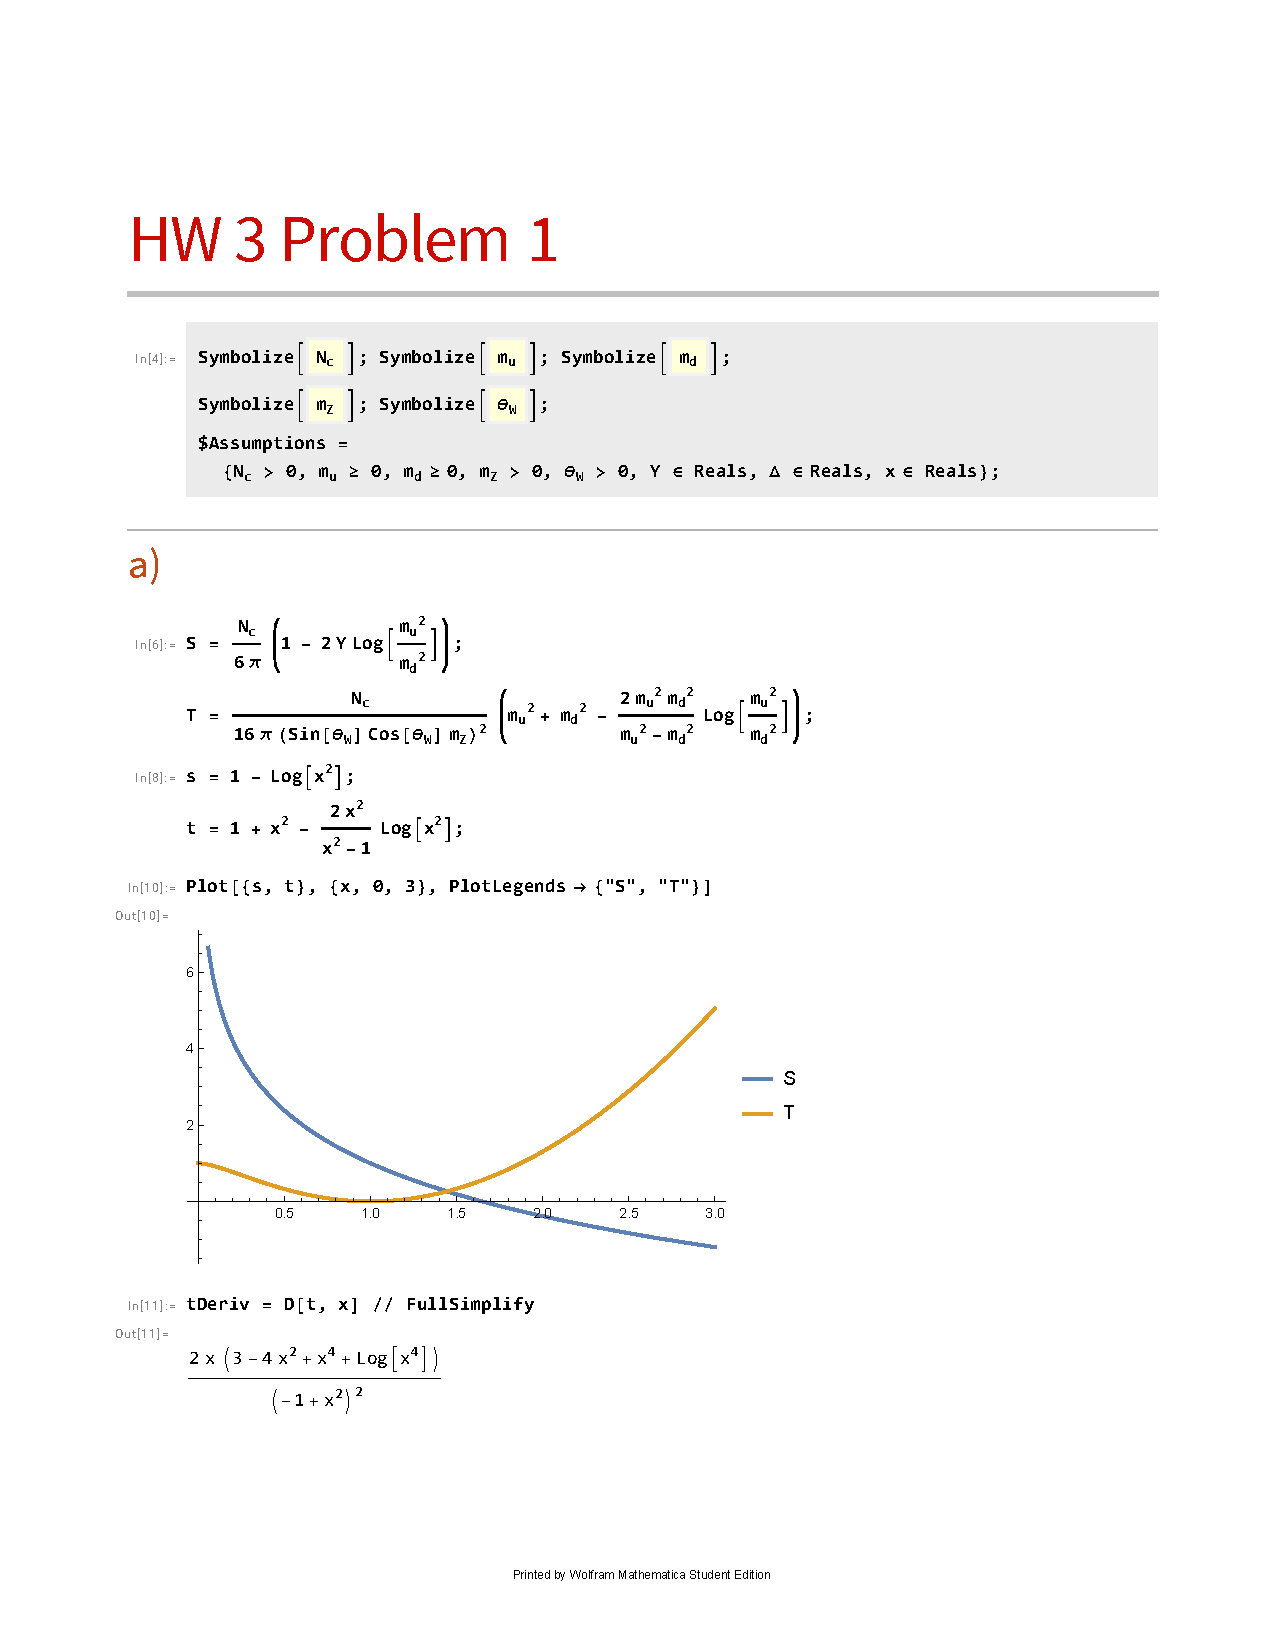
\includepdf[pages=-]{calcs/prob1.pdf}
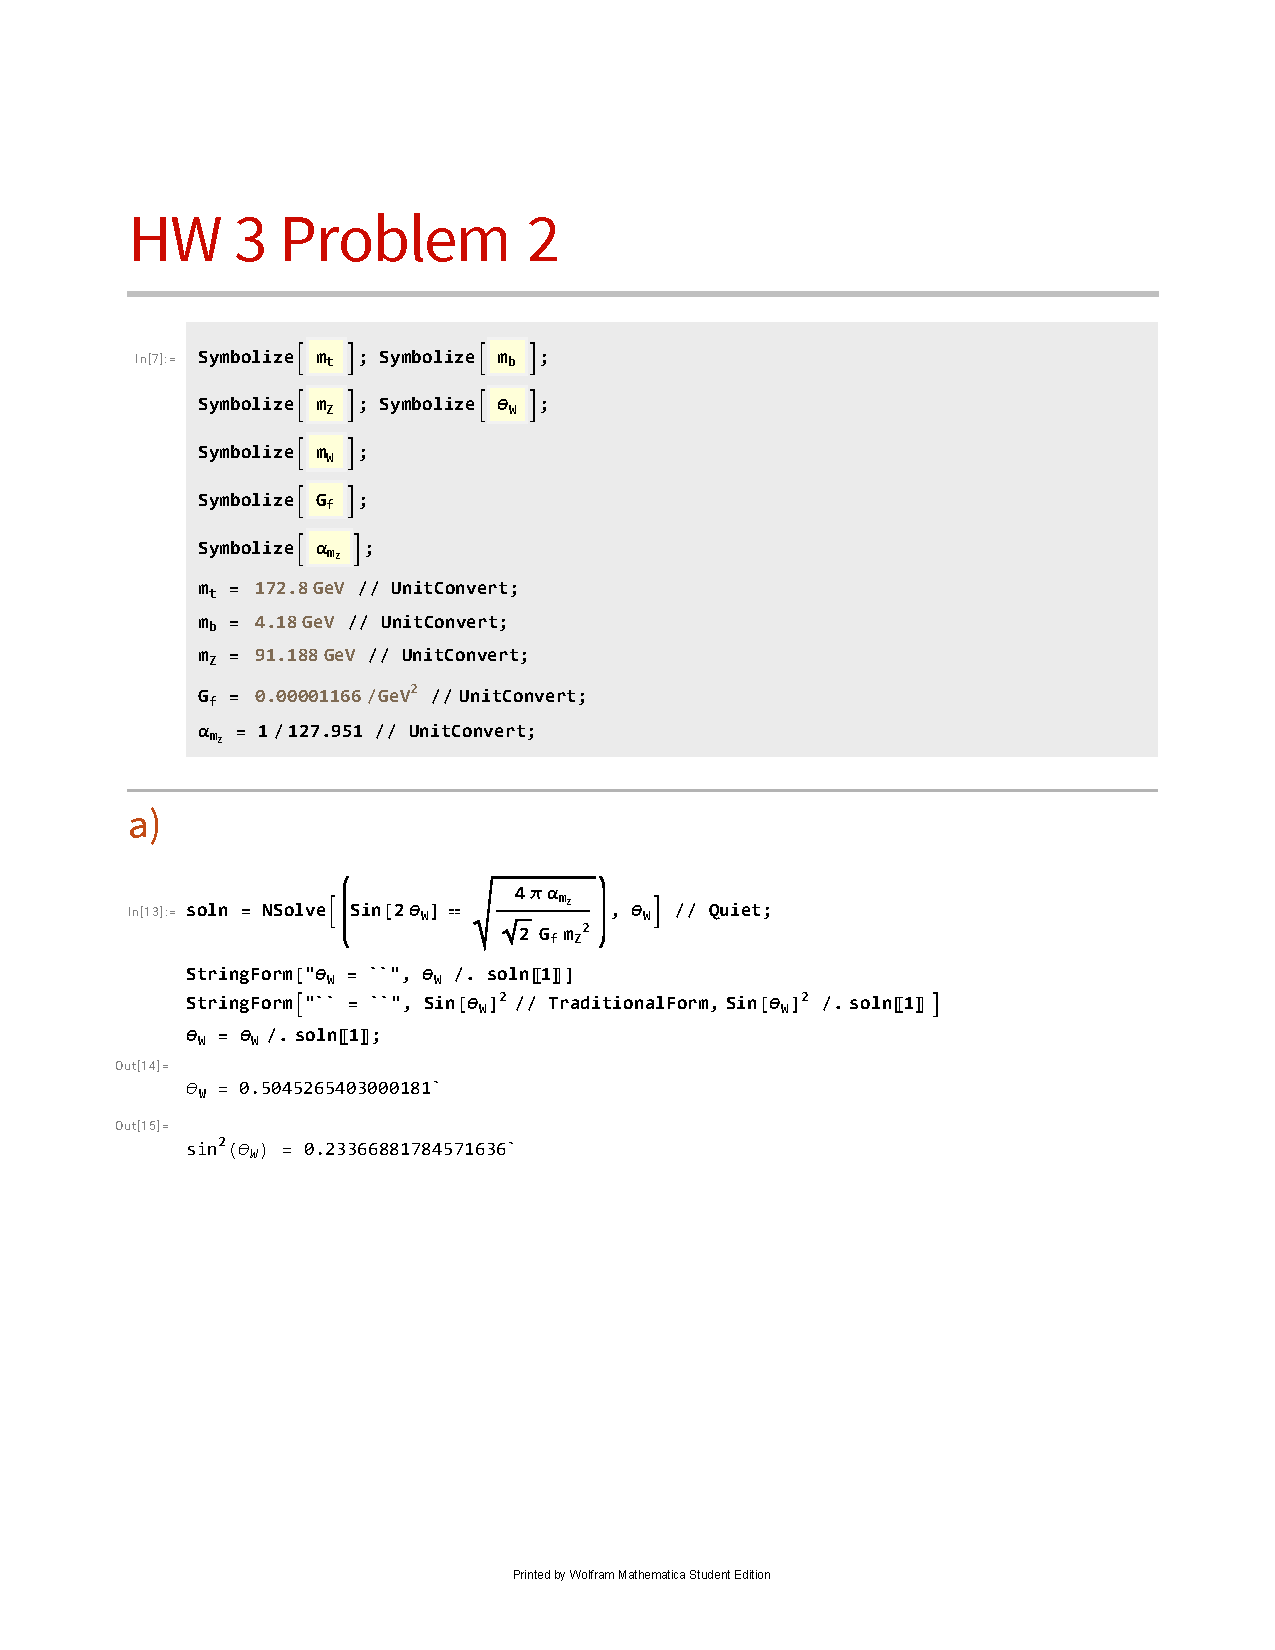
\includepdf[pages=-]{calcs/prob2.pdf}

\end{document}